% !TEX root = dissertationmain.tex
\chapter{Example Application Output}
\section{Fictional Small Network Output}
\label{fictional}
\paragraph{}This output was generated by running the application in automatic, verbosity level 2, twin input with graph plotting mode. The command used to execute the application with this configuration is as follows: 
\begin{lstlisting}[language=bash]
cluster.py -s automatic -vv -p -t -N -tp ../cw.xml ../cw.nessus
\end{lstlisting}
\paragraph{}The network in which the scans were taken place is an entirely fictional and uses four machines in the scope. This scope is described below.

\begin{table}[!h]
\centering
\caption{Fictional Network Scope and Machine Descriptions}
\label{fictional_scope}
\begin{tabular}{ll}
\hline
192.168.0.1  & \begin{tabular}[c]{@{}l@{}}Windows 2008 server running Apache 2 web server with MySQL database. \\ Hosting a DNS server.\\ Domain Controller for UADTARGETNET domain \\ running Lightweight Directory Access Protocol\\ NETBIOS name: SERVER1\end{tabular} \\
\hline
192.168.0.2  & \begin{tabular}[c]{@{}l@{}}Windows 2008 server \\ running empty web server and hosting a DNS server\\ running Lightweight Directory Access Protocol\\ NETBIOS name: SERVER2\end{tabular}                                                                   \\
\hline
192.168.0.10 & \begin{tabular}[c]{@{}l@{}}Windows 7 Professional 7600 (Windows 7 Professional 6.1)\\ NETBIOS name: CLIENT1\end{tabular}                                                                                                                                   \\
\hline
192.168.0.11 & \begin{tabular}[c]{@{}l@{}}Windows 7 Professional 7600 (Windows 7 Professional 6.1)\\ NETBIOS name: CLIENT2\end{tabular}                                                                                                                                  
\end{tabular}
\end{table}


\subsection{Text Output}
\label{exampleoutput}

\lstdefinestyle{lineoutput}
{
    language=bash,
    backgroundcolor=\color{white},
    basicstyle=\scriptsize\color{black}\ttfamily
}


\begin{lstlisting}[style=lineoutput]
04-19 01:32 19624 cluster <module> DEBUG    :twin flag enabled
04-19 01:32 19624 cluster <module> DEBUG    :tp: ../cw.xml , path: ['../cw.nessus']
04-19 01:32 19624 cluster <module> INFO     :Vectorizing Stage for Nessus
04-19 01:32 19624 parse_nessus parse_input INFO     :Parsing Nessus XML * BETA *
no of IP's taken from nessus: 4
04-19 01:32 19624 parse_nessus parse_input INFO     :Done Nessus parsing
04-19 01:32 19624 cluster <module> DEBUG    :Loaded 4 vectors with 45 features
04-19 01:32 19624 cluster <module> INFO     :Vectorizing complete

04-19 01:32 19624 cluster <module> INFO     :Vectorizing Stage for nmap
no of IP's taken from NMAP: 4
04-19 01:32 19624 cluster <module> DEBUG    :Loaded 4 vectors with 81 features
04-19 01:32 19624 cluster <module> INFO     :Vectorizing complete

04-19 01:32 19624 cluster <module> INFO     :Normalising the nessus vectors
04-19 01:32 19624 cluster <module> INFO     :Reducing vectors to two dimensions with PCA
04-19 01:32 19624 cluster <module> DEBUG    :reduced to 4 vectors with 2 dimensions
04-19 01:32 19624 cluster <module> INFO     :Normalising complete

04-19 01:32 19624 cluster <module> INFO     :Normalising the nmap vectors
04-19 01:32 19624 cluster <module> INFO     :Reducing vectors to two dimensions with PCA
04-19 01:32 19624 cluster <module> DEBUG    :reduced to 4 vectors with 2 dimensions
04-19 01:32 19624 cluster <module> INFO     :Normalising complete

04-19 01:32 19624 cluster <module> INFO     :Clustering Nessus
04-19 01:32 19624 cluster cluster DEBUG    :Starting prospective KMeans clusterings
04-19 01:32 19624 cluster cluster DEBUG    :Trying kmeans(n_clusters=2)
04-19 01:32 19624 cluster cluster DEBUG    :Trying kmeans(n_clusters=3)
04-19 01:32 19624 cluster cluster INFO     :Best clustering method: kmeans(n_clusters=2) (adjusted silhouette == 0.176059056707)
04-19 01:32 19624 cluster <module> INFO     :Clustering Complete


04-19 01:32 19624 cluster <module> INFO     :Clustering Nmap
04-19 01:32 19624 cluster cluster DEBUG    :Starting prospective KMeans clusterings
04-19 01:32 19624 cluster cluster DEBUG    :Trying kmeans(n_clusters=2)
04-19 01:32 19624 cluster cluster DEBUG    :Trying kmeans(n_clusters=3)
04-19 01:33 19624 cluster cluster INFO     :Best clustering method: kmeans(n_clusters=2) (adjusted silhouette == 0.441640409673)
04-19 01:33 19624 cluster <module> INFO     :Clustering Complete


Note: shared features does not retain keys from XML and therefore wont always be human readable.
Printing Nessus cluster details

Cluster ID: 0
Silhouette Score: 0.299967117317
IPs: 192.168.0.10, 192.168.0.11

    Shared Features:
    general-purpose
    windows
    445
    cpe:/o:microsoft:windows_7:::professional
    Mon Apr 03 11:25:23 2017
    Microsoft Windows 7 Professional
    9
    5355

 
 
Cluster ID: 1
Silhouette Score: 0.0521509960965
IPs: 192.168.0.1, 192.168.0.2

    Shared Features:
    Mon Apr 03 11:25:06 2017
    cpe:/o:microsoft:windows
    general-purpose
    windows
    53
    23
    445

 
 
cluster ID : amount of IP's
0 : 2
1 : 2



Printing Nmap cluster details

Cluster ID: 0
Silhouette Score: 0.213624573736
IPs: 192.168.0.1, 192.168.0.2

    Shared Features:
    tcp23opentelnet
    tcp42opentcpwrapped
    tcp53opendomain
    tcp80openhttp
    tcp88openkerberos-sec
    tcp135open
    tcp139open
    tcp389open
    tcp445open
    tcp464open
    tcp593open
    tcp636opentcpwrapped
    tcp3268open
    tcp3269opentcpwrapped
    tcp49152open
    tcp49153open
    tcp49154open
    tcp49155open
    tcp49157open
    tcp49158open

 
 
Cluster ID: 1
Silhouette Score: 0.66965624561
IPs: 192.168.0.10, 192.168.0.11

    Shared Features:
    tcp135openmsrpcMicrosoft Windows RPC
    tcp139opennetbios-ssnMicrosoft Windows 98 netbios-ssn
    tcp445openmicrosoft-dsMicrosoft Windows 10 microsoft-ds
    tcp49152openmsrpcMicrosoft Windows RPC
    tcp49153openmsrpcMicrosoft Windows RPC
    tcp49154openmsrpcMicrosoft Windows RPC
    tcp49175openmsrpcMicrosoft Windows RPC
    tcp49176openmsrpcMicrosoft Windows RPC

 
 
cluster ID : amount of IP's
0 : 2
1 : 2
04-19 01:33 19624 cluster <module> DEBUG    :Getting centroids using reduced vectors for Nmap:
04-19 01:33 19624 cluster <module> DEBUG    :nclusters: 2
04-19 01:33 19624 clustering get_centroids DEBUG    :K = 0

04-19 01:33 19624 cluster <module> DEBUG    :attempting to plot the following centroids:
 [[-0.56736301 -0.01841586]
 [ 0.56736301  0.01841586]]


04-19 01:33 19624 cluster <module> DEBUG    :Getting centroids using reduced vectors for Nessus:
04-19 01:33 19624 cluster <module> DEBUG    :nclusters: kmeans(n_clusters=2)
04-19 01:33 19624 cluster <module> DEBUG    :nclusters: 2
04-19 01:33 19624 clustering get_centroids DEBUG    :K = 0

04-19 01:33 19624 cluster <module> DEBUG    :attempting to plot the following centroids:
 [[-0.49416507 -0.0089938 ]
 [ 0.49416507  0.0089938 ]]


04-19 01:33 19624 cluster <module> INFO     :Nmap Centroids Covariance Matrix:
 [[ 0.64380156  0.02089695]
 [ 0.02089695  0.00067829]]
04-19 01:33 19624 cluster <module> INFO     :Nessus Centroids Covariance Matrix:
 [[  4.88398234e-01   8.88884549e-03]
 [  8.88884549e-03   1.61776945e-04]]
04-19 01:33 19624 cluster <module> INFO     :distance matrix between centroids using metric for Nmap: euclidean :
-------  -------
0        1.13532
1.13532  0
-------  -------
04-19 01:33 19624 cluster <module> INFO     :distance matrix between centroids using metric for Nessus: euclidean :
--------  --------
0         0.988494
0.988494  0
--------  --------
04-19 01:33 19624 cluster <module> INFO     :IP's from clusters with less than 3 IP's:
 ['192.168.0.1' '192.168.0.10' '192.168.0.11' '192.168.0.2']
04-19 01:33 19624 cluster <module> DEBUG    :Loaded 4 vectors with 126 features
04-19 01:33 19624 cluster <module> INFO     :Normalizing input and reducing vectors to two dimensions with PCA
04-19 01:33 19624 cluster <module> INFO     :Resulting single IP vectors:
 [[-0.50300301 -0.49063882]
 [ 0.52888708 -0.00269094]
 [ 0.56066029  0.03834554]
 [-0.58654436  0.45498422]]
04-19 01:33 19624 cluster <module> INFO     :distance matrix between centroids of small combined clusters: euclidean :
--------  ---------  ---------  --------
0         1.14144    1.18794    0.949306
1.14144   0          0.0518992  1.20568
1.18794   0.0518992  0          1.22052
0.949306  1.20568    1.22052    0
--------  ---------  ---------  --------
04-19 01:33 19624 clustering cluster_single_kmeans INFO     :Calculating gap statistic value, this can take a while...

04-19 01:33 19624 clustering cluster_single_kmeans INFO     :gap statistics recommends number of clusters: 3

04-19 01:33 19624 clustering cluster_single_kmeans DEBUG    :No K value specified, using Gap Statistic

04-19 01:33 19624 cluster <module> INFO     :Writing recommended attack IP's to targets.txt for exploitation
 {0}
04-19 01:33 19624 display twin DEBUG    :twin cluster plot.
04-19 01:33 19624 single_ip_parsing_nmap parse_input DEBUG    :found ip 192.168.0.1
04-19 01:33 19624 single_ip_parsing_nmap parse_input DEBUG    :found ip 192.168.0.2
04-19 01:33 19624 single_ip_parsing_nmap parse_input DEBUG    :found ip 192.168.0.10
04-19 01:33 19624 single_ip_parsing_nmap parse_input DEBUG    :found ip 192.168.0.11
04-19 01:33 19624 display twin DEBUG    :{'192.168.0.2': ['"Microsoft Windows 7 SP0 - SP1, Windows Server 2008 SP1, Windows 8, or Windows 8.1 Update 1. Prediction accuracy: 100"'], '192.168.0.1': [], '192.168.0.10': ['"Microsoft Windows 7 SP0 - SP1, Windows Server 2008 SP1, Windows 8, or Windows 8.1 Update 1. Prediction accuracy: 100"'], '192.168.0.11': ['"Microsoft Windows 7 SP0 - SP1, Windows Server 2008 SP1, Windows 8, or Windows 8.1 Update 1. Prediction accuracy: 100"']}
\end{lstlisting}

\subsection{Graphing Interface Output}
\label{example_twin}

\paragraph{}The Figure \ref{example_twin} below shows the example graphing interface output using the configuration mentioned previously in Appendix \ref{fictional}.

\begin{figure}[!h]
\centering
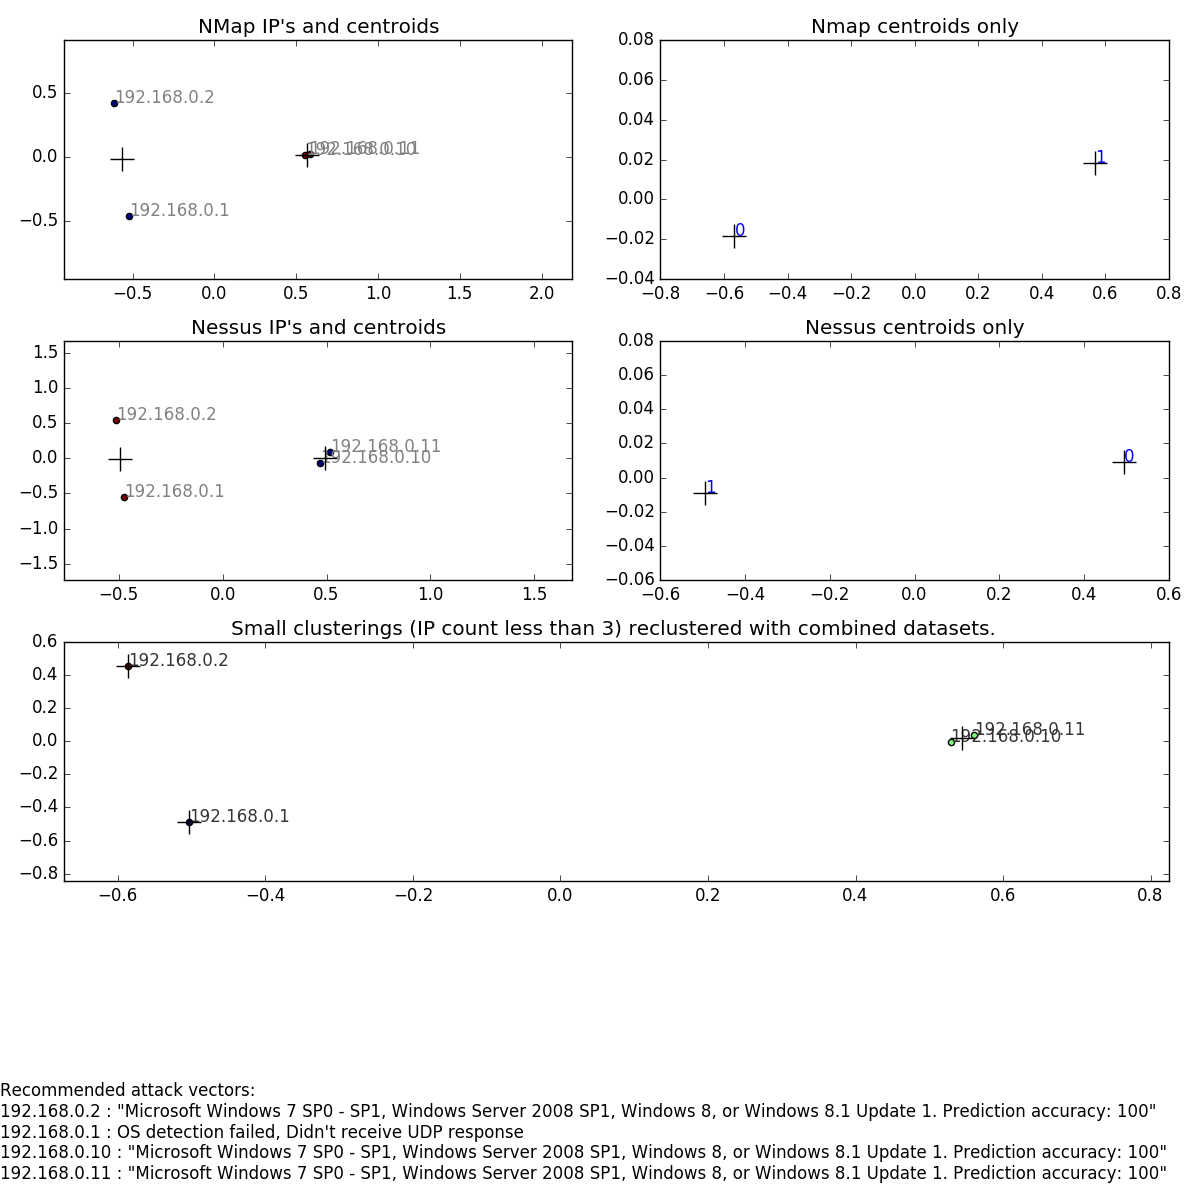
\includegraphics[width=6in]{./Figures/example_twin.png}
\caption{Example of graphing interface GUI from a fictional network to be used in conjunction with text output at \ref{examplesoutput}}
\label{example_twin}
\end{figure}
